%%%%%%%%%%%%%%%%%%%%%%%%%%%%%%%%%%%%%%%%%%%%%%%%%%%%%%%%%%%%%%%%%%%%%%%%%%%%%%%%
%2345678901234567890123456789012345678901234567890123456789012345678901234567890
%        1         2         3         4         5         6         7         8

\documentclass[letterpaper, 10 pt, conference]{ieeeconf}  % Comment this line out
                                                          % if you need a4paper
%\documentclass[a4paper, 10pt, conference]{ieeeconf}      % Use this line for a4
                                                          % paper

\IEEEoverridecommandlockouts                              % This command is only
                                                          % needed if you want to
                                                          % use the \thanks command
\overrideIEEEmargins
% See the \addtolength command later in the file to balance the column lengths
% on the last page of the document



% The following packages can be found on http:\\www.ctan.org
% \usepackage{graphics} % for pdf, bitmapped graphics files
\usepackage{graphicx}
\graphicspath{ {./data/} }
% \usepackage{subcaption}
\usepackage{amsmath}
\usepackage{float}
\usepackage{subfig}
\usepackage{listings}
\usepackage[skipbelow=\topskip,skipabove=\topskip]{mdframed}
% \usepackage{subfig}
%\usepackage{epsfig} % for postscript graphics files
%\usepackage{mathptmx} % assumes new font selection scheme installed
%\usepackage{times} % assumes new font selection scheme installed
%\usepackage{amsmath} % assumes amsmath package installed
%\usepackage{amssymb}  % assumes amsmath package installed

\title{\LARGE \bf
Assignment 1 : Image Editor 
}

%\author{ \parbox{3 in}{\centering Huibert Kwakernaak*
%         \thanks{*Use the $\backslash$thanks command to put information here}\\
%         Faculty of Electrical Engineering, Mathematics and Computer Science\\
%         University of Twente\\
%         7500 AE Enschede, The Netherlands\\
%         {\tt\small h.kwakernaak@autsubmit.com}}
%         \hspace*{ 0.5 in}
%         \parbox{3 in}{ \centering Pradeep Misra**
%         \thanks{**The footnote marks may be inserted manually}\\
%        Department of Electrical Engineering \\
%         Wright State University\\
%         Dayton, OH 45435, USA\\
%         {\tt\small pmisra@cs.wright.edu}}
%}

\author{Saqib Azim - 150070031% <-this % stops a space
% \thanks{*This work was not supported by any organization}% <-this % stops a space
% \thanks{$^{1}$H. Kwakernaak is with Faculty of Electrical Engineering, Mathematics and Computer Science,
%         University of Twente, 7500 AE Enschede, The Netherlands
%         {\tt\small h.kwakernaak at papercept.net}}%
% \thanks{$^{2}$P. Misra is with the Department of Electrical Engineering, Wright State University,
%         Dayton, OH 45435, USA
%         {\tt\small p.misra at ieee.org}}%
}


\begin{document}
\maketitle
\thispagestyle{empty}
\pagestyle{empty}

%%%%%%%%%%%%%%%%%%%%%%%%%%%%%%%%%%%%%%%%%%%%%%%%%%%%%%%%%%%%%%%%%%%%%%%%%%%%%%%%
\begin{abstract}

This report describes the layout, features, functionalities and results of a GUI image editor implemented in Python. This image editor is easy-to-use and portable across different computer devices.
\end{abstract}

%%%%%%%%%%%%%%%%%%%%%%%%%%%%%%%%%%%%%%%%%%%%%%%%%%%%%%%%%%%%%%%%%%%%%%%%%%%%%%%%
\section{\textbf{INTRODUCTION}}
The entire Graphical User Interface has been designed and implemented using Python's library - PyQt (version 5)
The basic layout of the GUI is divided in three sections : \\
1. Original Image Grid : Always displays image loaded \\
2. Modified Image Grid : Displays the modified image as a result of user interaction  \\
3. User Handle Grid : Includes various image manipulation buttons for performing operations on image \\

The User Handle Grid consists of following buttons : \\
1. Load Image : select an image from an input dialog box \\
2. Histogram Equalize : \\
3. Gamma Correction  \\
4. Log Transform  \\
5. Image Blur using Gaussian Kernel  \\ 
6. Image Sharpening using "Unsharp Masking"  \\
7. Special Feature - Canny Edge Detection   \\
8. Undo the last operation performed on image  \\
9. Undo all the operations performed on the image loaded and display the last image loaded \\
10. Save the modified image  \\
11. Close \& Exit the Image Editor  \\

\section{\textbf{Background Reading}}
\begin{itemize}
\item PyQt Library
\item Edge Detection Using Canny Edge Detection Technique
\item Histogram Equalization
\item Image Sharpening using Unsharp Masking
\end{itemize}

\section{\textbf{Approach}}
The image editor window has been allowed to take the entire desktop available (Full-Screen Mode). The entire layout is shown in fig. 1
\begin{figure}[h!]%
	\centering
    \subfloat[]{{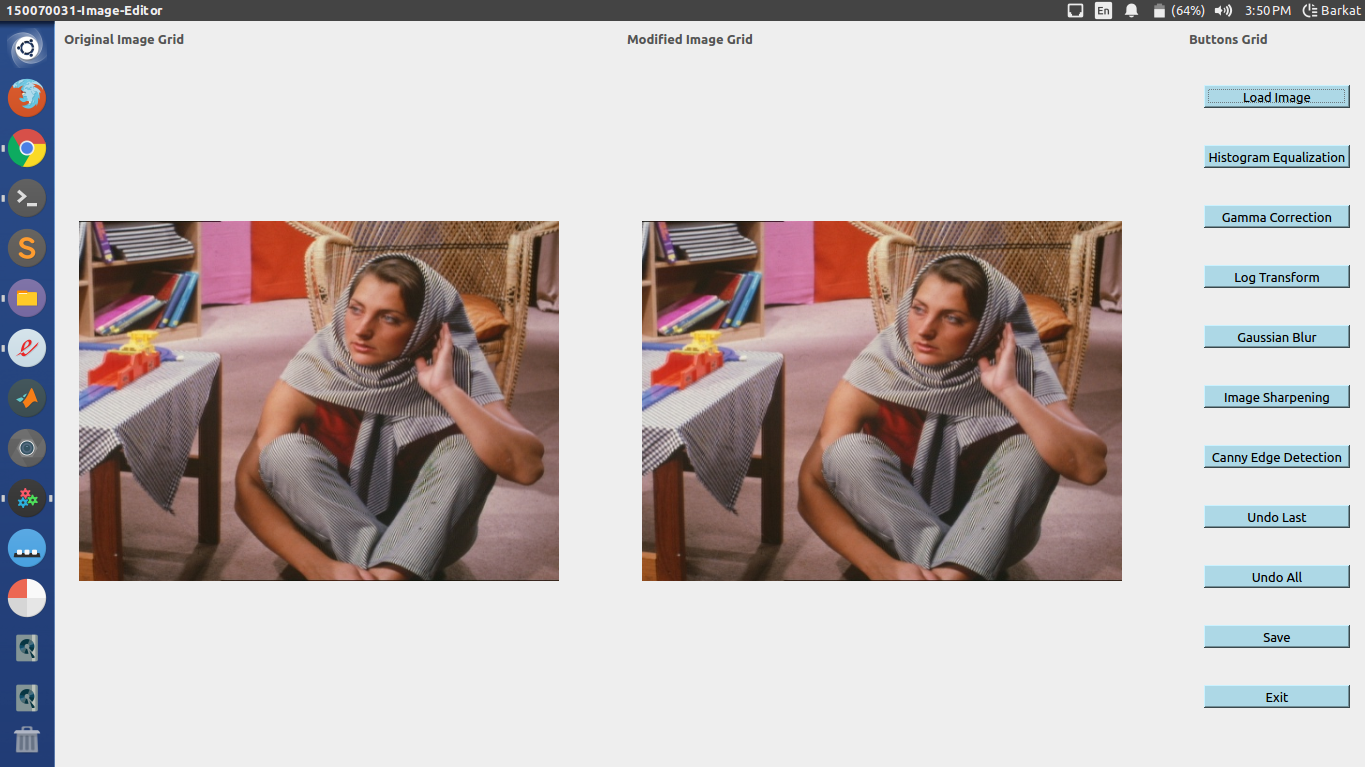
\includegraphics[width=7cm,height=4cm]{window}}}%
    \caption{Image Editor Window Layout}%
    \label{fig:image_editor_layout}%
\end{figure}

\subsection{\textbf{Image Loading}}
On clicking the "Load Image" pushbutton, a file selector dialog box appears which will display and process the file only if it is an image file (*.png, *.jpg, *.jpeg etc). If the user selects a file other than an image file, a warning message will pop-up. \\
Upon image loading, it is first converted from BGR to HSV format and all further operations are done using only the V-channel (except special feature case of canny Edge Detection where all three channels RGB are used) with H,S channel untouched/unchanged.

\subsection{\textbf{Histogram Equalization}}
The steps for computing histogram equalization are described as follows :\\
1. Find the histogram of input image \\
2. Compute the cumulative distribution from histogram computed in step I \\
3. Compute the probability distribution and scale it by multiplying with 255 \\
4. Create a new zero-filled image for storing output image
5. Assign the new intensity values to pixels based on the pdf computed. Let T be the transformation function, L the number of intensity levels, $p_r$ probability distribution computed in step 3.
\[s_{k} = T(r_{k}) = (L-1)\sum_{j=0}^{k}p_r(r_j) \] 

\subsection{\textbf{Gamma Correction and Log Transform}}
Both the features have similar implementations. The input image is normalized to [0-1] range. In gamma correction, gamma-value is user-input and the scale factor c in both cases has been set to 1. After the respective operation, the image is brought back to [0-255] range. \\
Gamma Correction Transformation : s is output image intensity, r is input image intensity, c and $\gamma$ are parameters \[ s = cr^{\gamma}\] Log Transform : s is output image intensity, r is input image intensity, c is tunable parameter\[ s = c\ln(1+r) \]

\subsection{\textbf{Image Blurring}}
Blurring is implemented using Gaussian Kernel. The kernel is computed based on the user provided kernel size (W) and standard deviation ($\sigma$) of the gaussian kernel
\[K(x, y) = \frac{1}{2\pi \sigma^2}\exp({-\frac{x^2 + y^2}{2\sigma^2}}) \]. The kernel is normalized by dividing it by sum of all kernel elements so that total sum of the kernel elements is 1. 
\[ K(x, y) = \frac{K(x, y)}{\sum_{i=0}^{W-1}\sum_{j=0}^{W-1}K(i, j)} \]A check has been imposed for restricting the kernel dimensions (W) to be an odd integer. The image to be blurred is zero-padded first for convolving with kernel. One disadvantage of padding zeros which is observed is the darkening of boundary pixels in blurred image. 

\subsection{\textbf{Image Sharpening}}
"Unsharp Masking" has been used for sharpening the image. For this input image is first blurred using Gaussian kernel of fixed kernel size (W) = 5 and standard deviation ($\sigma$) = 2 and the resultant blurred image is subtracted from input image to get mask. Let F be the input image, G be the gaussian kernel and M be the mask image then, 
\[M = F - G*F\]
To get the sharpened image, input image is added to a scaled version of mask Image where scale parameter is user-input. O is the output image and s is the scale parameter.
\[O = F + s\times mask \]
\[O = F + s\times(F - G*F)\]

\subsection{\textbf{Special Features - Canny Edge Detector} }
The steps for finding the edges using Canny Edge Detection method are as follows :
\begin{itemize}
\item Input image blurred using gaussian kernel of fixed window size (W) = 3 and standard deviation ($\sigma$) = 1.6 to reduce noise
\item Gradient magnitude  of blurred image is computed at each pixel in x \& y directions by convolving with gradient kernel 
\[ K_{x} = \begin{bmatrix}
    -1 & 0 & 1 \\
    -2 & 0 & 2 \\
    -1 & 0 & 1
  \end{bmatrix} 
  K_{y} = \begin{bmatrix}
    1 & 2 & 1 \\
    0 & 0 & 0 \\
    -1 & -2 & -1
  \end{bmatrix}\]
  \[ G = \sqrt[]{G_{x}^2 + G_{y}^2}\]
\item The pixels where the gradient magnitude is greater than neighbours along gradient direction is marked
\item Those pixels where gradient magnitude is greater than a threshold (upperThreshold) are selected and connected path is found out starting from selected pixels where all pixels have gradient magnitude greater than lower threshold.
\end{itemize}

\subsection{\textbf{Undo the Last Operation Performed}}
Since all the operations are performed on the V-channel with H,S channel unchanged, following steps are taken for implementing this feature :
\begin{itemize}
\item The present V-channel image is combined with its corresponding H,S channels
\item The HSV image is converted to RGB and stored in a temporary variable
\item The previous image variable(which stores the previous image) is converted from RGB->HSV and its V-channel stored in present image variable (which is displayed on screen)
\item Display the previous image variable
\item The temporary variable is assigned to previous image variable
\item [Steps 1-5] Swapping the present image and previous image using temporary variable
\end{itemize}

\subsection{\textbf{Undo All changes and Revert to Loaded Image}}
Following Steps are performed for this feature :
\begin{itemize}
\item The present V-channel image is combined with its corresponding H,S channels
\item The HSV image converted to RGB and stored in previous image variable
\item The original loaded image converted to HSV and its V-channel stored in present image variable
\item The original image displayed
\end{itemize}

\subsection{\textbf{Saving the present modified image}}
On clicking the save button, a dialog box appears for the user to select the location of image to be saved. The present image is saved by first converting HSV format to RGB and saving using openCV. 

\section{\textbf{Selection \& Results on Test Images}}
\subsection{\textbf{Histogram Equalization}}
This feature will be more dominant/useful in those images which have non-uniform histogram distribution (for example, dark image where most of the pixels have lower intensity or very light image where most of the pixels have high intensity). Hence the testing images were either very dark or lighted where histogram equalization will result in more information (visually) in output image compared to input image
\begin{figure}[h!]%
	\centering
    \subfloat[Input Image]{{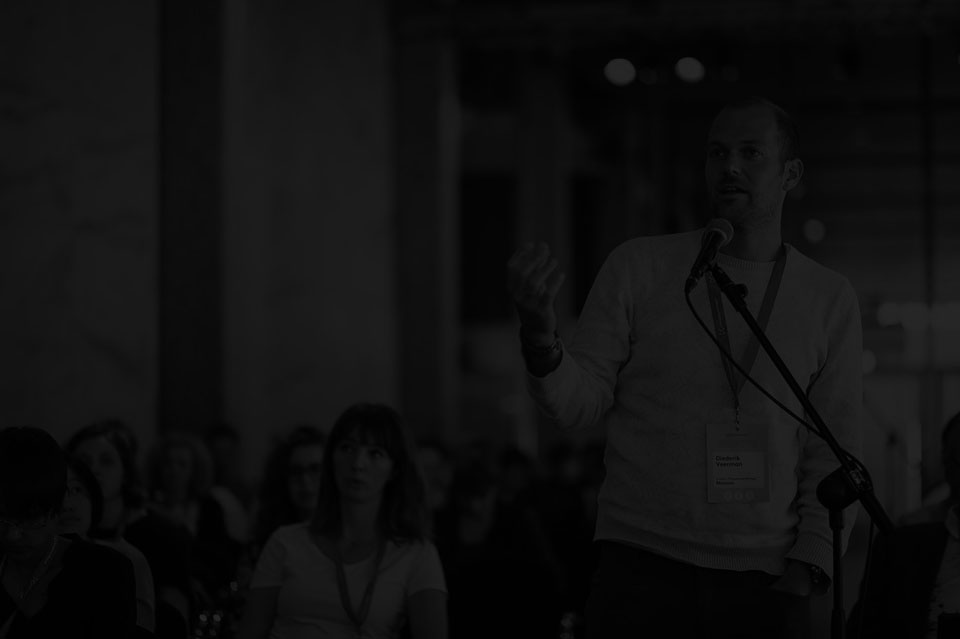
\includegraphics[width=3.5cm,height=3cm]{histEqualized1}}}%
    \qquad
    \subfloat[Histogram Equalized Image]{{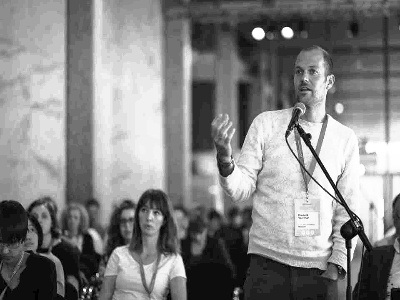
\includegraphics[width=3.5cm, height=3cm]{histEqualized1_result} }}%
    \caption{Comparison of input and histogram equalized image}%
    \label{fig:example}%
\end{figure}

\begin{figure}[h!]%
	\centering
    \subfloat[Histogram of input image]{{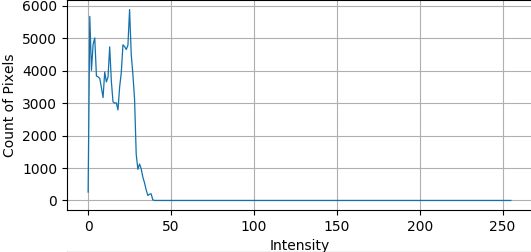
\includegraphics[width=3.5cm,height=3cm]{histEqualized1_plot1}}}%
    \qquad
    \subfloat[Histogram of Output image]{{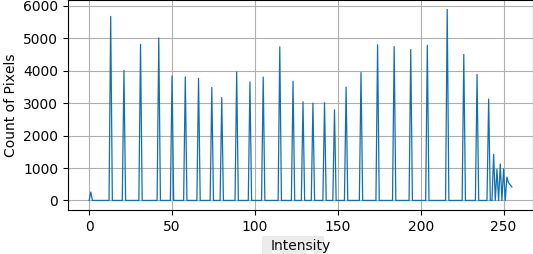
\includegraphics[width=3.5cm, height=3cm]{histEqualized1_plot2} }}%
    \caption{Histogram of input and histogram equalized image}%
    \label{fig:example}%
\end{figure}
\begin{figure}[h!]%
	\centering
    \subfloat[Input Image]{{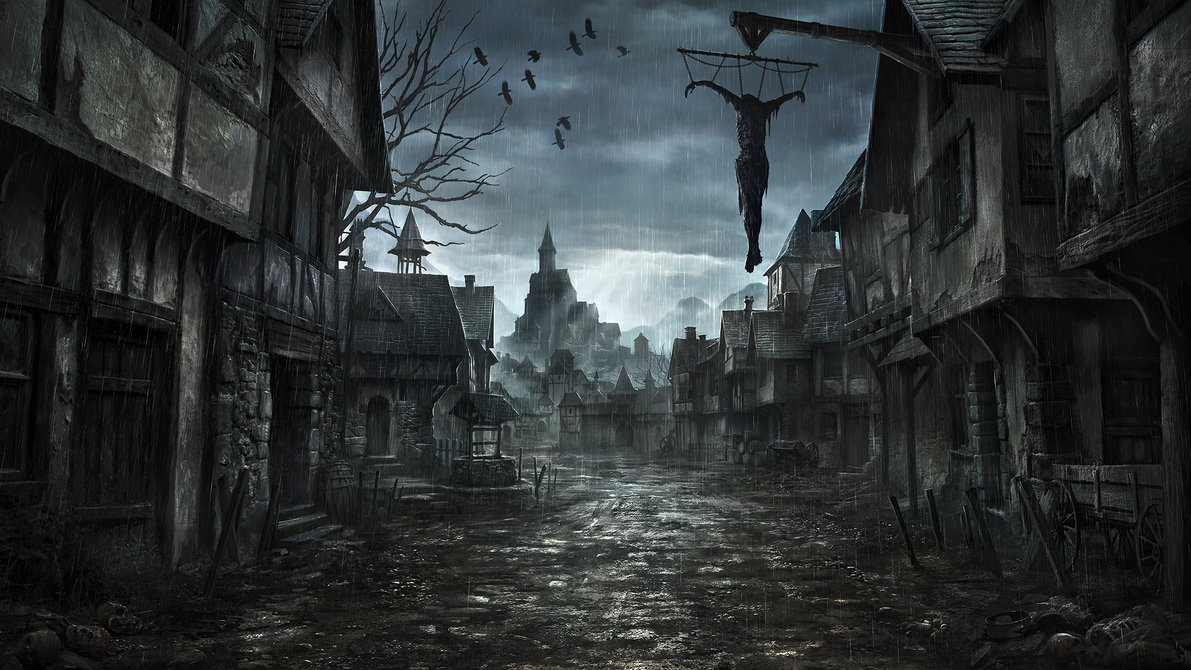
\includegraphics[width=3.5cm,height=3cm]{darkAges}}}%
    \qquad
    \subfloat[Histogram Equalized Image]{{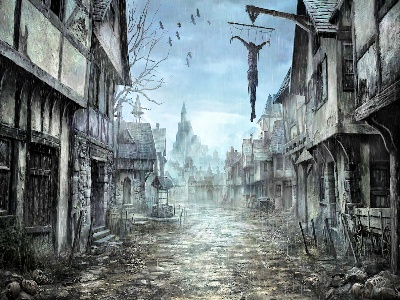
\includegraphics[width=3.5cm, height=3cm]{darkAges_histEqualize} }}%
    \caption{Comparison of input and histogram equalized image}%
    \label{fig:histogram_equalize1}%
\end{figure}

\begin{figure}[h!]%
	\centering
    \subfloat[Histogram of input image]{{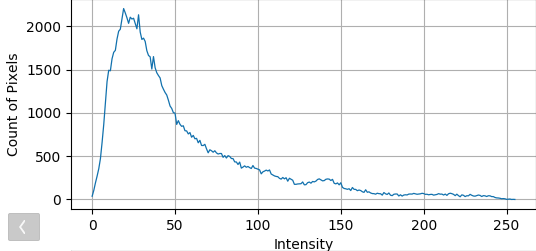
\includegraphics[width=3.5cm,height=3cm]{darkAges_plot1}}}%
    \qquad
    \subfloat[Histogram of Output image]{{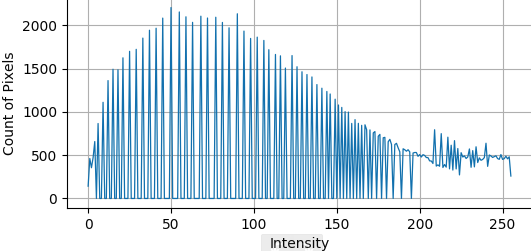
\includegraphics[width=3.5cm, height=3cm]{darkAges_plot2} }}%
    \caption{Histogram of input and histogram equalized image}%
    \label{fig:histogram_equalize2}%
\end{figure}



\subsection{\textbf{Gamma Transformation}}
In gamma tranform, taking $\gamma < 1$ will result in darker intensity pixels getting stretched resulting in overall image looking brighter compared to input image. On the other hand taking $\gamma > 1$ results in higher intensities getting streched making the overall image look darker compared to input image. 

\begin{figure}[h!]%
	\centering
    \subfloat[Input Image]{{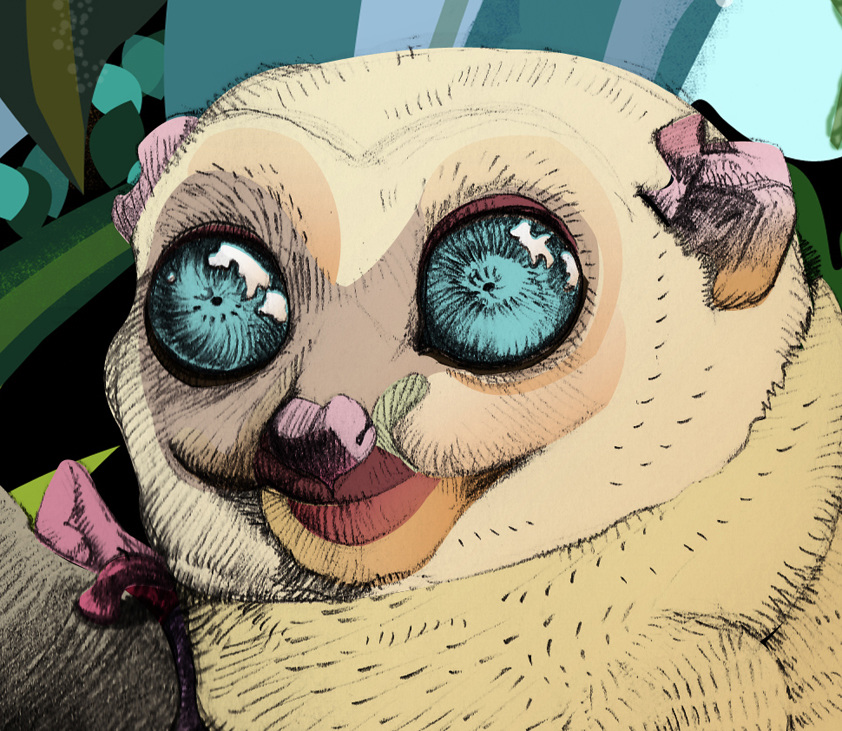
\includegraphics[width=3.5cm,height=3cm]{monkey2}}}%
    \qquad
    \subfloat[Gamma Corrected Image (gamma=0.2)]{{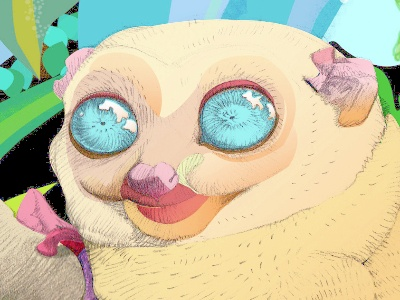
\includegraphics[width=3.5cm, height=3cm]{monkey2_gamma_correction1} }}%
    \caption{Results of Gamma Correction}%
    \label{fig:gamma_correction1}%
\end{figure}
\begin{figure}[h!]%
	\centering
    \subfloat[Input Image]{{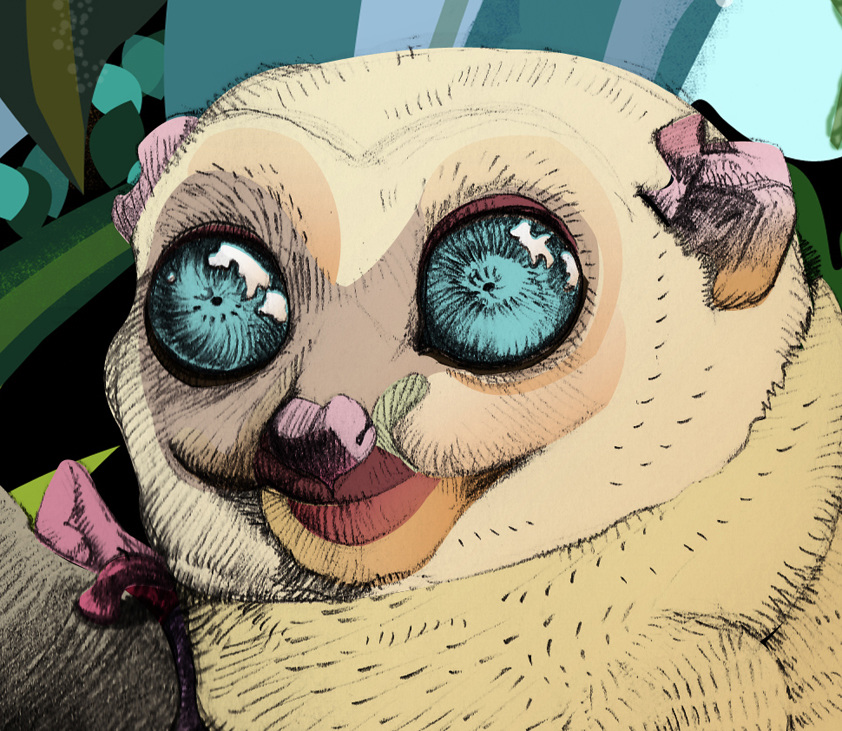
\includegraphics[width=3.5cm,height=3cm]{monkey2}}}%
    \qquad
    \subfloat[Gamma Corrected Image (gamma=3.0)]{{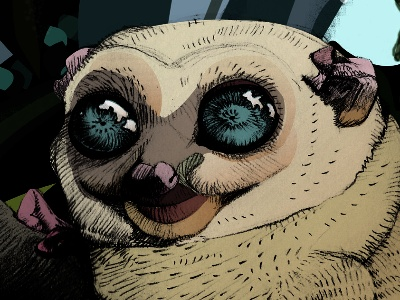
\includegraphics[width=3.5cm, height=3cm]{monkey2_gamma_correction_3} }}%
    \caption{Results of Gamma Correction}%
    \label{fig:gamma_correction2}%
\end{figure}

\subsection{\textbf{Log Transformation}}
This transformation results in darker pixels getting stretched in intensity making the overall image look brighter compared to input image. Hence the input image is a darker image with some information not visible to naked eyes but after doing the transformation the image becomes more pleasing to the eyes. 

\begin{figure}[h!]%
	\centering
    \subfloat[Input Image]{{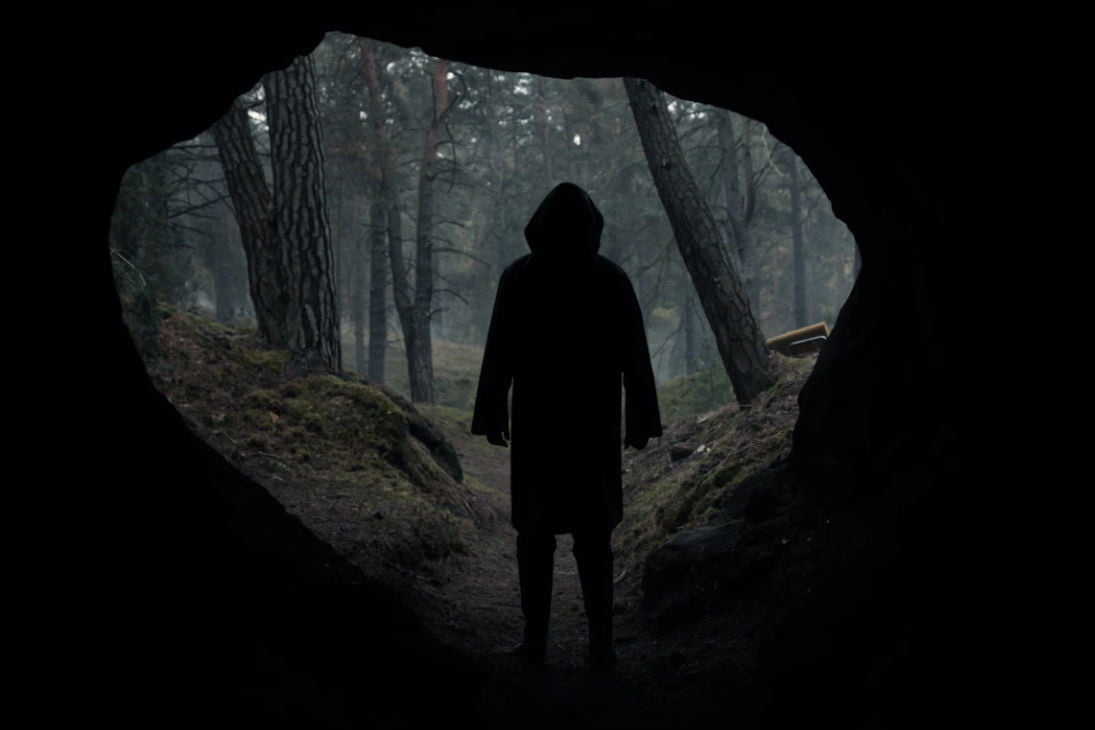
\includegraphics[width=3.5cm,height=3cm]{darkImage}}}%
    \qquad
    \subfloat[Log Transform(5 times)]{{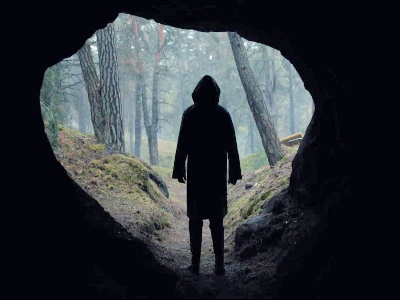
\includegraphics[width=3.5cm, height=3cm]{darkImage_log_transform_5} }}%
    \caption{Results of Log Transform}%
    \label{fig:log_transform}%
\end{figure}

\subsection{\textbf{Image Blurring}}
The results of blurring will be most prominent in sharp images with lot of texture details or edge information and also in images with noise. Hence both the images chosen here give a distinctive idea of the extent of blurring. 

\begin{figure}[h!]%
	\centering
    \subfloat[Input Image]{{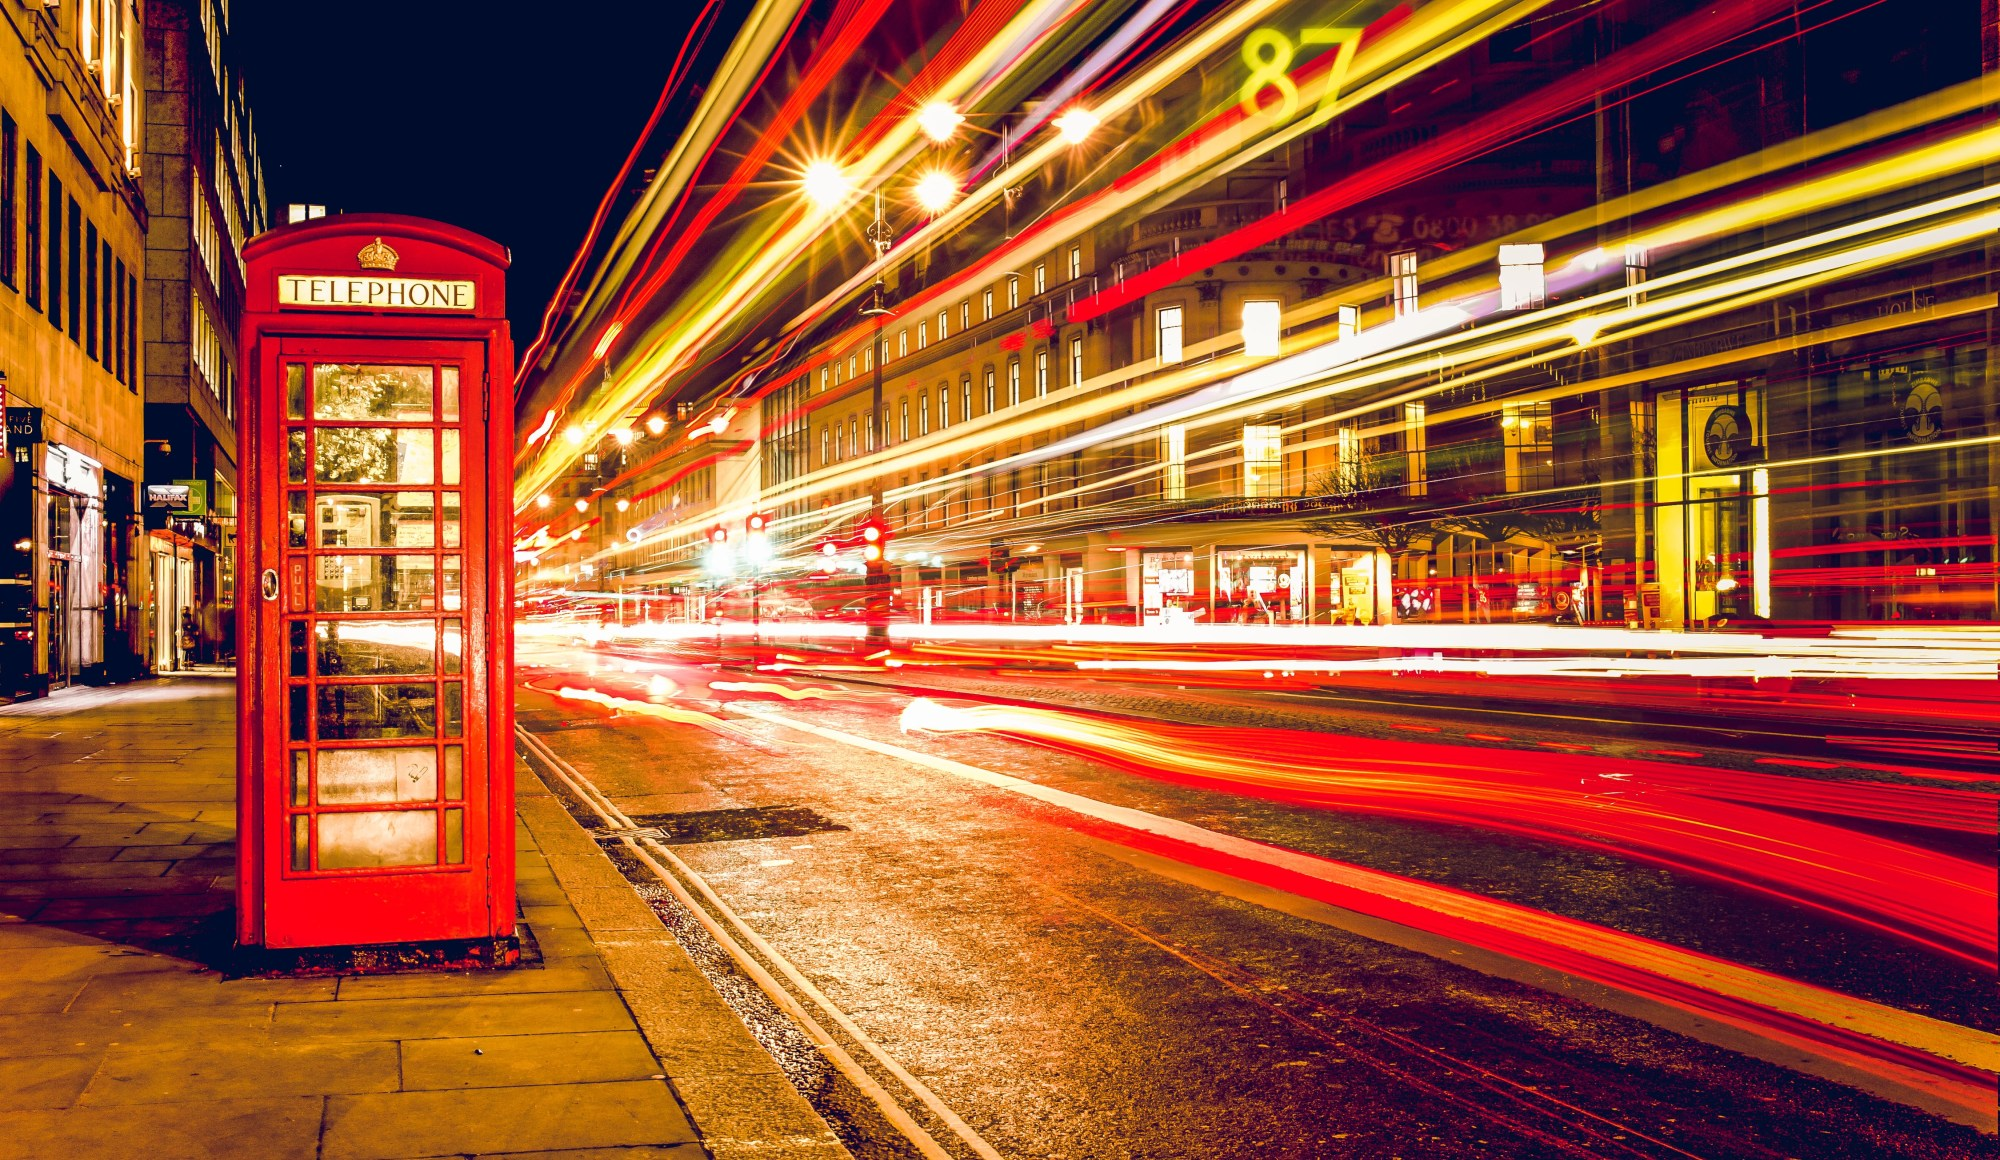
\includegraphics[width=3.5cm,height=3cm]{citylights}}}%
    \qquad
    \subfloat[Gaussian Blurred Image (W=11, sigma=4)]{{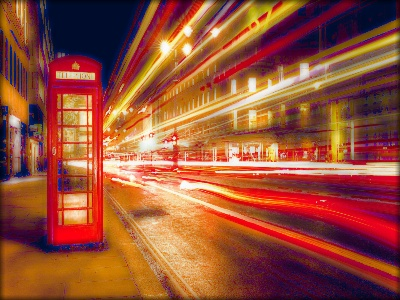
\includegraphics[width=3.5cm, height=3cm]{citylights_blurred} }}%
    \caption{Results of Gaussian Blurring}%
    \label{fig:image_blur1}%
\end{figure}

\begin{figure}[h!]%
	\centering
    \subfloat[Input Image]{{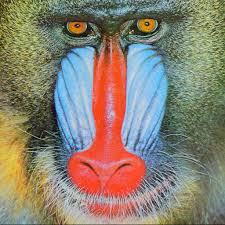
\includegraphics[width=3.5cm,height=3cm]{monkey}}}%
    \qquad
    \subfloat[Gaussian Blurred Image (W=7, sigma=5)]{{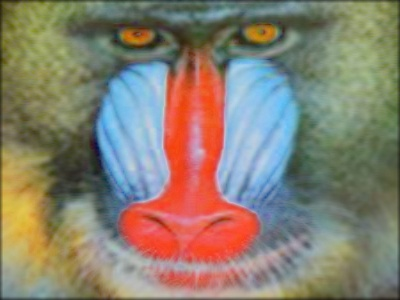
\includegraphics[width=3.5cm, height=3cm]{monkey_blurred} }}%
    \caption{Results of Gaussian Blurring}%
    \label{fig:image_blur2}%
\end{figure}

\subsection{\textbf{Image Sharpening}}
Image sharpening in vague terms is a high pass filter and will be most effective in blurred images. Hence both the testing images are blurred and result in images with more visual information content compared to input image. 

\begin{figure}[h!]%
	\centering
    \subfloat[Input Image]{{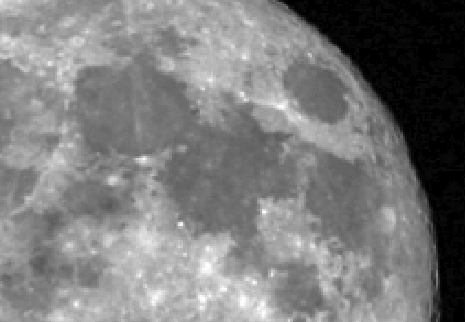
\includegraphics[width=3.5cm,height=3cm]{moon}}}%
    \qquad
    \subfloat[Sharpened Image (scale factor k=3)]{{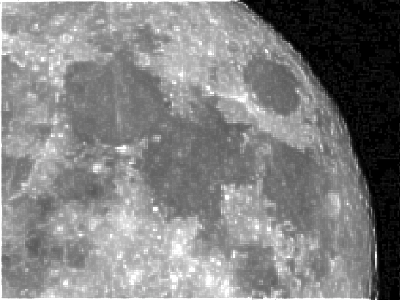
\includegraphics[width=3.5cm, height=3cm]{moon_sharpened} }}%
    \caption{Results of Image Sharpening}%
    \label{fig:image_sharp1}%
\end{figure}

\begin{figure}[h!]%
	\centering
    \subfloat[Input Image]{{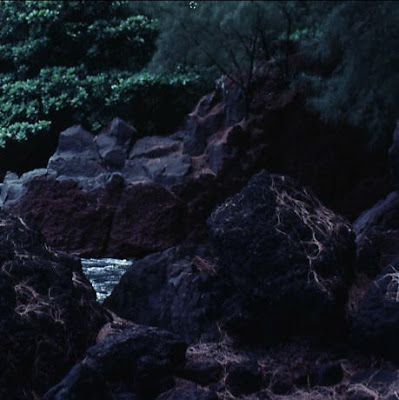
\includegraphics[width=3.5cm,height=3cm]{rock}}}%
    \qquad
    \subfloat[Sharpened Image (scale factor k=7)]{{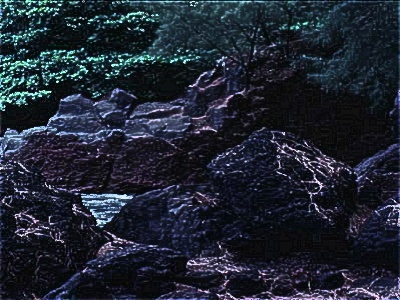
\includegraphics[width=3.5cm, height=3cm]{rock_sharpened} }}%
    \caption{Results of Image Sharpening}%
    \label{fig:image_sharp2}%
\end{figure}

\subsection{\textbf{Canny Edge Detection}}
Choosing testing images for this feature was more intuitive compared to other features. The images having distinctive edges and textures serve the purpose of test images.

\begin{figure}[h!]%
	\centering
    \subfloat[Input Image]{{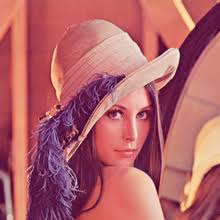
\includegraphics[width=3.5cm,height=3cm]{lena}}}%
    \qquad
    \subfloat[Canny Edge Detected Image (lt=20, ut=40)]{{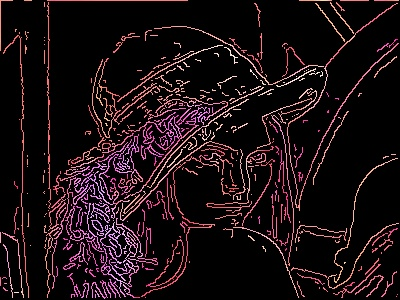
\includegraphics[width=3.5cm, height=3cm]{lena_ced} }}%
    \caption{Results of Canny Edge Detector}%
    \label{fig:canny_edge_detector1}%
\end{figure}

\begin{figure}[h!]%
	\centering
    \subfloat[Input Image]{{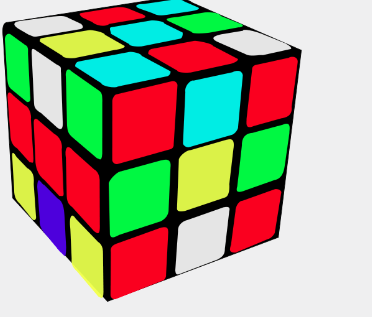
\includegraphics[width=3.5cm,height=3cm]{rubiksCube}}}%
    \qquad
    \subfloat[Canny Edge Detected Image (lt=20, ut=40)]{{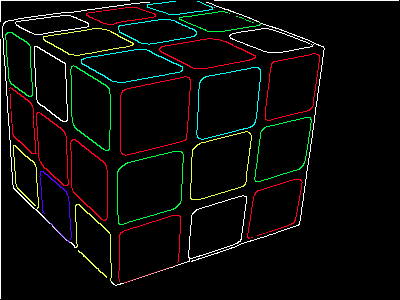
\includegraphics[width=3.5cm, height=3cm]{rubiksCube_ced} }}%
    \caption{Results of Canny Edge Detector}%
    \label{fig:canny_edge_detector2}%
\end{figure}

\section{\textbf{Discussion and Challenges faced}}
\begin{itemize}
\item While implementing image sharpening, the image convolved with gaussian kernel need to be subtracted from input image forming the mask image. Also the mask image needs to be added to input image. Using numpy subtraction and addition causes wrap-around effect (for example, 5-10 leads to 251). This was solved by using openCV subtraction and addition which clips negative values to zero.
\item The most difficult problem faced was to use QPixmap to display images. The QPixmap documentation for displaying images is not very rich leading to various problems like converting image from opencv format to QImage format since QPixmap only takes QImage format as argument

\end{itemize}
\subsection{\textbf{Future Steps/Things which could have done if more time was there}}
\begin{itemize}
\item The histogram plot could have been fit inside the main editor window
\item Implement another method of Image sharpening - Laplacian or Using Sobel operators and compare Unsharp Masking with Laplacian based sharpening
\end{itemize}

% \section*{APPENDIX}

% Appendixes should appear before the acknowledgment.

\begin{thebibliography}{99}
\bibitem{c1} R. C. Gonzalez, R. E. Woods, Digital Image Processing, 3rd ed. Prentice Hall
\bibitem{c2} S.W.Awate, Segmentation-Edge Detection, Lecture Notes, Digital Image Processing
\bibitem{c3} A.Sethi, Intensity Transform and Spatial Filtering, Lecture Notes
\bibitem{c4} Canny Edge Detector Code - https://github.com/fubel/PyCannyEdge
\bibitem{c5} PyQt5 Official Website - https://pythonspot.com/pyqt5/
\bibitem{c6} PyQt5 Tutorials Point - https://www.tutorialspoint.com/pyqt/index.htm
\bibitem{c7} Convert openCV Image to QImage - https://gist.github.com/smex/5287589
\bibitem{c8} Open QMainWindow in Full Screen Window - https://www.qtcentre.org/threads/4662-Open-a-QMainWindow-in-full-screen-mode
\bibitem{c9} Insert images in Latex - https://www.latex-tutorial.com/tutorials/figures/
\bibitem{c10} \textbf{Github Link to code} - https://github.com/saqib1707/Image-Editor/blob/master/main.py
\end{thebibliography}

\onecolumn
\section{Appendix}
\subsection{main.py}
\begin{mdframed}
\begin{lstlisting}
import sys,cv2
import numpy as np
import matplotlib.pyplot as plt
from PyQt5.QtWidgets import QApplication, QWidget, QPushButton, QLabel, QMessageBox, QInputDialog, QFileDialog, QHBoxLayout, QGroupBox, \
                            QDialog, QVBoxLayout, QGridLayout,QLineEdit
from PyQt5.QtCore import pyqtSlot, Qt
from PyQt5.QtGui import QPixmap, qRgb, QImage

gray_color_table = [qRgb(i, i, i) for i in range(256)]

def generateGaussianKernel(winSize, sigma):
    """
        generates a gaussian kernel taking window size = winSize
        and standard deviation = sigma as input/control parameters. 

        Returns the gaussian kernel
    """
    kernel = np.zeros((winSize, winSize))        # generate a zero numpy kernel
    for i in range(winSize):
        for j in range(winSize):
            temp = pow(i-winSize//2,2)+pow(j-winSize//2,2)
            kernel[i,j] = np.exp(-1*temp/(2*pow(sigma,2)))
    kernel = kernel/(2*np.pi*pow(sigma,2))
    norm_factor = np.sum(kernel)               # finding the sum of the kernel generated
    kernel = kernel/norm_factor                # dividing by total sum to make the kernel matrix unit-sum
    return kernel

def boxKernel(winSize):
    """
        returns  a box kernel with window size = winSize
    """
    kernel = np.ones((winSize, winSize))/(winSize*winSize)
    return kernel

def roundAngle(angle):
    """ 
        this functions rounds-off the input angle to four values
        Input angle must be in [0,180) 
    """
    # converts angle in radian to degree
    angle = np.rad2deg(angle) % 180
    if (0 <= angle < 22.5) or (157.5 <= angle < 180):
        angle = 0
    elif (22.5 <= angle < 67.5):
        angle = 45
    elif (67.5 <= angle < 112.5):
        angle = 90
    elif (112.5 <= angle < 157.5):
        angle = 135
    return angle


class MyImageEditor(QWidget):
    def __init__(self):
        super().__init__()
        self.title = '150070031-Image-Editor'               # declare the title of editor window
        self.left = 100                                     # (next two lines) x-y co-ordinate on the screen where the editor's top left corner will lie
        self.top = 100 
        self.width = 840                                    # the width and height of the editor window
        self.height = 480
        self.number_horizontal_box_layouts = 3
        self.initUserInterface()                            # initialize the User Interface
 
    
    def initUserInterface(self):
        self.setWindowTitle(self.title)                     # sets window title as defined above
        geometry = myApp.desktop().availableGeometry()        # window size = entire screen available
        # self.setGeometry(self.left, self.top, self.width, self.height)  # sets the geometry of the window
        self.setGeometry(geometry)                          # sets the geometry of the window

        self.createGridLayout()
        windowLayout = QHBoxLayout()

        for i in range(self.number_horizontal_box_layouts):
            windowLayout.addWidget(self.horizontalGroupBox[i])
        self.setLayout(windowLayout)                   # sets the layout of editor-window to be windowLayout
        self.show()                                    # displays the editor-window on screen

        self.label = QLabel(self)                     # initialize pyqt QLabel widget for displaying original Image always
        self.label_result = QLabel(self)                      # QLabel widget for displaying modified Image after each \
                                                    # operation. Initialized to original Image in the beginning 

        self.layout[0].addWidget(self.label)                               # both the label widgets declared above added to 1st & 2nd layout resp.                             
        self.layout[1].addWidget(self.label_result)

    
    def createGridLayout(self):
        self.layout = []                               # initialize layout of the editor-window to be an empty list
        number_layouts = 3                             # first layout : for showing the original image \
                                                       # sedond layout : for showing the modified image \
                                                       # third layout : for all the pushbuttons 
        for i in range(number_layouts):
            self.layout.append(QGridLayout())          # each layout type is GridLayout.Creates a gridlayout object and appends to layout list

        self.layout[0].setColumnStretch(1, 2)
        self.layout[1].setColumnStretch(1, 2)
 
        nButtons = 11                                  # number of buttons
        buttonLabel = ['Load Image', 'Histogram Equalization', 'Gamma Correction', 'Log Transform', 'Gaussian Blur', 'Image Sharpening', 'Canny Edge Detection', 
                       'Undo Last', 'Undo All', 'Save', 'Exit']          # Labels of pushbutton
        onButtonClick = [self.loadImage, self.histEqualize, self.gammaCorrection, self.logTransform, self.blurImage, self.sharpImage, 
                        self.specialFeature, self.undoLast, self.undoAll, self.saveImage, self.myExit]    # list of functions that are executed when the 
                                                                                                # corresponding button defined in buttonLabel is clicked
        buttons = []                                             # an empty list created for storing pushbutton objects
        for i in range(nButtons):
            buttons.append(QPushButton(buttonLabel[i], self))    # Pushbutton object created with the first argument as the button label \
                                                                 # and appended in the buttons list
            buttons[i].clicked.connect(onButtonClick[i])         # Pushbutton attached with an event listener which results in corresponding \
                                                                 # function in onButtonClick list to be executed on button click
            buttons[i].setStyleSheet("color : black; background-color : lightblue;")  # sets the button text color and background color
            self.layout[2].addWidget(buttons[i],i,0)             # Pushbutton object added to layout 3 at position (i,0)

        horizontalGroupBox_Label = ["Original Image Grid", "Modified Image Grid", "Buttons Grid"]
        self.horizontalGroupBox = []
        for i in range(self.number_horizontal_box_layouts):
            self.horizontalGroupBox.append(QGroupBox(horizontalGroupBox_Label[i]))
            self.horizontalGroupBox[i].setLayout(self.layout[i])

    
    def finalDisplay(self, result):
        """
            Display Image
            Input argument 
                result : two dimensional image/single channel
        """
        # combine V-channel (self.image) with H,S channel
        self.hsvImage[:,:,2] = self.image
        self.prevImage = cv2.cvtColor(self.hsvImage, cv2.COLOR_HSV2RGB)
        self.hsvImage[:,:,2] = result
        # update the image display with the modified HSV image
        qImage = self.convertCvToQImage(cv2.cvtColor(self.hsvImage, cv2.COLOR_HSV2RGB))
        self.label_result.setPixmap(QPixmap(qImage))
        self.image = result

    
    def openFileNameDialog(self):
        fileLoadOptions = QFileDialog.Options()
        fileLoadOptions |= QFileDialog.DontUseNativeDialog
        fileName, _ = QFileDialog.getOpenFileName(self, "Load Image File","","All Files (*);;jpg (*.jpg);; png (*.png)", options = fileLoadOptions)
        possibleImageTypes = ['jpg', 'png', 'jpeg', 'bmp']                             # only these image extensions are allowed

        if (fileName and (fileName.split('.')[1] in possibleImageTypes)):       # if user selects a file and it is a allowed file
            self.origImage = cv2.resize(cv2.imread(fileName, 1), (480, 360))    # reads a color image. Resizes to (image_width, image_height)=(400, 300)
            self.origImage = cv2.cvtColor(self.origImage, cv2.COLOR_BGR2RGB)    # openCV image color format when reading = BGR (by default) and \
                                                                                # converts image format from BGR to RGB for later convenience
            self.prevImage = self.origImage                                     # previous image variable for "Undo to Last" Operation
            self.hsvImage = cv2.cvtColor(self.origImage, cv2.COLOR_RGB2HSV)     # convert image format from RGB -> HSV for operations on V channel
            self.image = self.hsvImage[:, :, 2].astype(np.uint8)                # self.image = V channel of original HSV image
            qImage = self.convertCvToQImage(self.origImage)                     # convert openCV image -> pyQt QImage for displaying in Pixmap
            # set pixmap with the original loaded image in both original and modified grids
            self.label.setPixmap(QPixmap(qImage))
            self.label_result.setPixmap(QPixmap(qImage))
            # self.label_result.setPixmap(None)
        elif (fileName):                                                        # case when user selects a file with extension not in "possibleImageTypes"
            buttonReply = QMessageBox.question(self, 'Warning Message', "Wrong File Selection", QMessageBox.Ok, QMessageBox.Ok)


    
    def convertCvToQImage(self, img, copy=False):
        """
            converts opencv image to QImage. 
            source : Stack Overflow
            Input : img must be in openCV image format (np.uint8)
        """
        if img is None:
            return QImage()
        # if input image format is openCv image format np.uint8
        if img.dtype == np.uint8:
            # grayscale image or images having two dimensions [height, width]
            if len(img.shape) == 2:
                qim = QImage(img.data, img.shape[1], img.shape[0], img.strides[0], QImage.Format_Indexed8)
                qim.setColorTable(gray_color_table)
                return qim.copy() if copy else qim
            # image having three dimansions [height, width, nChannels]
            elif len(img.shape) == 3:
                # if image has three channels
                if img.shape[2] == 3:
                    qim = QImage(img.data, img.shape[1], img.shape[0], img.strides[0], QImage.Format_RGB888)
                    return qim.copy() if copy else qim
                # if image has four channels
                elif img.shape[2] == 4:
                    qim = QImage(img.data, img.shape[1], img.shape[0], img.strides[0], QImage.Format_ARGB32)
                    return qim.copy() if copy else qim

    
    @pyqtSlot()
    def loadImage(self):
        self.openFileNameDialog()             # [In-Built Function] opens a dialog box for user to choose an Image

    
    @pyqtSlot()
    def histEqualize(self):
        """
            Histrogram Equalization Function
                1. finds the histogram of input image
                2. computes the cumulative distribution of input image
                3. computes the probability distribution and scale it to 255
                4. assign the new intensity values to pixels
                5. Plots the input image histogram and equalized image histogram 
        """
        L = 256
        imgHeight, imgWidth = self.image.shape
        resultantImage = np.zeros(self.image.shape)                          # numpy array of zeros for output "histogram equalized" image
        original_img_hist = np.zeros((L, 1))                                  # variable to store the input image histogram
        equalized_img_hist = np.zeros((L, 1))                                 # variable to store the "histogram equalized" image histogram
        for i in range(L):                                                   # compute the histogram of input image
            original_img_hist[i, 0] = np.sum(self.image == i)

        cdf = np.zeros(original_img_hist.shape)
        sumHist = 0
        for i in range(L):
            sumHist = sumHist + original_img_hist[i,0]                    # finds the cumulative distribution of input image
            cdf[i,0] = sumHist
        # cdf = np.cumsum(original_img_hist)                                   
        temp = ((L-1)/(imgHeight*imgWidth))                                       # temporary variable
        for i in range(L):                                                   # compute the transform values for each intensity from [0-255] and assign it
            resultantImage[np.where(self.image == i)] = np.round(temp*cdf[i])# to the pixels locations where that intensity is present in input image
        for i in range(L):                                                
            equalized_img_hist[i, 0] = np.sum(resultantImage == i)            # compute the histogram of output image
        resultantImage = resultantImage.astype(np.uint8)                     # change output image type for display purposes

        # the following lines plots the input and output image histograms in a (6x6) plot window
        fig = plt.figure(1, figsize = (6, 6))
        plt.subplot(211); plt.plot(original_img_hist, linewidth=0.9); plt.xlabel('Intensity'); plt.ylabel('Count of Pixels'); plt.grid(True)
        plt.subplot(212); plt.plot(equalized_img_hist, linewidth=0.9); plt.xlabel('Intensity'); plt.ylabel('Count of Pixels'); plt.grid(True)
        plt.suptitle('Comparison of Original vs Equalized Image Histograms')
        plt.show()

        self.finalDisplay(resultantImage)                                    # display the output image          


    
    @pyqtSlot()
    def gammaCorrection(self):
        c = 1.0
        gamma, okPressed = QInputDialog.getDouble(self, "Get Gamma Value", "Value:")               # dialog-box for taking gamma value as input
        if okPressed:                                                                              # if user presses "OK" only then only compute 
            normImage = cv2.normalize(self.image.astype('float'), None, 0.0, 1.0, cv2.NORM_MINMAX) # convert image from [0-255] -> [0-1]
            resultantImage = c*pow(normImage, gamma)                                               # output image = c*(input image)^gamma
            max_result = np.max(resultantImage)                                                    # finding the maximum intensity value  of output image
            resultantImage = (resultantImage/max_result)*255.0                                     # bring the output image to [0-255] range
            resultantImage = resultantImage.astype(np.uint8)                                       # change output image type for display purposes
            self.finalDisplay(resultantImage)                                                            # display the output image 

    
    @pyqtSlot()
    def logTransform(self):
        # c, okPressed = QInputDialog.getDouble(self, "C Value", "Value:")
        # if okPressed:
        c = 1.0
        normImage = cv2.normalize(self.image.astype('float'), None, 0.0, 1.0, cv2.NORM_MINMAX)  # convert image from [0-255] -> [0-1]
        resultantImage = c*np.log(1+normImage)                                                  # output image = c*ln(1 + normalized_Image)
        max_result = np.max(resultantImage)                                                     # finding the maximum intensity value  of output image
        resultantImage = (resultantImage/max_result)*255.0                                      # bring the output image to [0-255] range
        resultantImage = resultantImage.astype(np.uint8)                                        # change output image type for display purposes
        self.finalDisplay(resultantImage)                                                       # display the output image

    
    @pyqtSlot()
    def blurImage(self):
        """
            Blur Image using Gaussian Kernel with kernel size and gaussian variance
            chosen by initUserInterface
        """
        winSize, ok1Pressed = QInputDialog.getInt(self, "Kernel Window Size", "Value (odd number > 0):")      # get gaussian kernel size from user
        sigma, ok2pressed = QInputDialog.getDouble(self, "Standard Deviation", "Value (> 0):")     # get variance of gaussian kernel from user
        if (ok1Pressed and ok2pressed):                                                     # if both "OK" pressed then proceed further
            if(winSize%2!=0):                                                               # if kernel size is odd number the proceed further \
                                                                                            # else display a warning message
                imgHeight, imgWidth = self.image.shape
                mykernel = generateGaussianKernel(winSize, sigma)                           # get gaussian kernel
                # mykernel = boxKernel(winSize)
                paddedImage = np.zeros((imgHeight+(winSize//2)*2, imgWidth+(winSize//2)*2), dtype=np.uint8)   # initialize an empty zero-padded image for \
                                                                                            # convolution with gaussian kernel
                paddedImage[winSize//2:imgHeight+winSize//2, winSize//2:imgWidth+winSize//2] = self.image     # replace the central section of padded image \
                                                                                                         # with input image
                blurredImage = np.zeros(self.image.shape,dtype=np.uint8)                       # initialize empty image of size=imagesize for storing result
                for i in range(imgHeight):                                                     # convolution of zero-padded image and gaussian kernel
                    for j in range(imgWidth):
                        blurredImage[i,j] = np.round(np.sum(paddedImage[i:i+winSize, j:j+winSize]*mykernel))   # since gaussian kernel is symmetric matrix \
                                                                                        # as well as diagonal-symmetric, convolution ~ matrix multiplication
                blurredImage = blurredImage.astype(np.uint8)                            # change output image type for display purposes
                self.finalDisplay(blurredImage)                                         # display the output image
            else:
                buttonReply = QMessageBox.question(self, 'Warning Message', "Kernel Size has to be an odd number", QMessageBox.Ok, QMessageBox.Ok)

    
    @pyqtSlot()
    def sharpImage(self):
        # k = scale factor in unsharp masking; user input
        k, okPressed = QInputDialog.getDouble(self, "Scale Factor (k)", "Value (default = 5):") 
        if okPressed is None:
            k = 5
        winSize = 5         # kernel size for gaussian blurring
        sigma = 2           # standard deviation for gaussian blurring
        imgHeight, imgWidth = self.image.shape
        # kernel window of given winSize and sigma
        mykernel = generateGaussianKernel(winSize, sigma)
        # zero padded image for convolution with gaussian kernel
        paddedImage = np.zeros((imgHeight+(winSize//2)*2, imgWidth+(winSize//2)*2), dtype=np.uint8)
        paddedImage[winSize//2:imgHeight+winSize//2, winSize//2:imgWidth+winSize//2] = self.image
        blurredImage = np.zeros(self.image.shape,dtype=np.uint8)
        for i in range(imgHeight):
            for j in range(imgWidth):
                # convolution operation
                blurredImage[i,j] = np.sum(paddedImage[i:i+winSize, j:j+winSize]*mykernel)    
        # scaled version of mask computed by subtracting the blurred image from original image and scaling by k
        maskImage = k*cv2.subtract(self.image, blurredImage)
        maskImage = maskImage.astype(np.uint8)
        # sharp image computed by adding scaled mask with original image
        sharpenedImage = cv2.add(self.image, maskImage)
        sharpenedImage = sharpenedImage.astype(np.uint8)
        # display the sharpened image 
        self.finalDisplay(sharpenedImage)

        
    @pyqtSlot()
    def specialFeature(self):
        """
            Canny Edge DEtection
            Source : https://github.com/fubel/PyCannyEdge
        """
        sigma = 1.6                      # standard deviation for gaussian blurring 
        winSize = 3                      # kernel size for gaussian blurring
        strong = np.int32(255)
        weak = np.int32(50)

        lowerThreshold, ok1Pressed = QInputDialog.getInt(self, "Lower Threshold", "Value (default = 20):")
        upperThreshold, ok2Pressed = QInputDialog.getInt(self, "Upper Threshold", "Value (default = 40):")

        if ok1Pressed:
            pass
        else:
            lowerThreshold = 20

        if ok2Pressed:
            pass
        else:
            upperThreshold = 40

        # combine V-channel (self.image) with H,S channel
        self.hsvImage[:,:,2] = self.image
        img = cv2.cvtColor(cv2.cvtColor(self.hsvImage, cv2.COLOR_HSV2BGR), cv2.COLOR_BGR2GRAY)
        img = img.astype(np.int32)
        imgHeight, imgWidth = img.shape

        mykernel = generateGaussianKernel(winSize, sigma)
        # zero padded image for convolution with gaussian kernel
        paddedImage = np.zeros((imgHeight+(winSize//2)*2, imgWidth+(winSize//2)*2), dtype=np.int32)
        paddedImage[winSize//2:imgHeight+winSize//2, winSize//2:imgWidth+winSize//2] = img
        blurredImage = np.zeros(self.image.shape,dtype=np.int32)
        for i in range(imgHeight):
            for j in range(imgWidth):
                blurredImage[i,j] = np.sum(paddedImage[i:i+winSize, j:j+winSize]*mykernel)
        # kernel for finding gradient in X & Y direction
        kernelGradientX = np.array([[-1, 0, 1], [-2, 0, 2], [-1, 0, 1]], np.int32)    # vertical edges
        kernelGradientY = np.array([[1, 2, 1], [0, 0, 0], [-1, -2, -1]], np.int32)    # horizontal edges

        paddedImage[winSize//2:imgHeight+winSize//2, winSize//2:imgWidth+winSize//2] = blurredImage
        # for storing the convolution result of 
        gradientX = np.zeros(img.shape, dtype=np.int32)
        gradientY = np.zeros(img.shape, dtype=np.int32)

        # convolution for finding gradients
        for i in range(imgHeight):
            for j in range(imgWidth):
                gradientX[i,j] = np.round(np.sum(paddedImage[i:i+winSize, j:j+winSize]*(-1*kernelGradientX)))
                gradientY[i,j] = np.round(np.sum(paddedImage[i:i+winSize, j:j+winSize]*(-1*kernelGradientY)))

        # gradientMagnitude = \sqrt(gx*gx + gy*gy)
        gradientMagnitude = np.hypot(gradientX, gradientY)
        gradientDirection = np.arctan2(gradientY, gradientX)

        # output image for displaying canny edges
        edgeDetectedImage = np.zeros((imgHeight, imgWidth), dtype=np.int32)

        for i in range(imgHeight):
            for j in range(imgWidth):
                # find neighbour pixels to visit from the gradient directions
                quantizedGradientDirection = roundAngle(gradientDirection[i, j])
                try:
                    if quantizedGradientDirection == 0:
                        if (gradientMagnitude[i, j] >= gradientMagnitude[i, j - 1]) and (gradientMagnitude[i, j] >= gradientMagnitude[i, j + 1]):
                            edgeDetectedImage[i,j] = gradientMagnitude[i,j]
                    elif quantizedGradientDirection == 90:
                        if (gradientMagnitude[i, j] >= gradientMagnitude[i - 1, j]) and (gradientMagnitude[i, j] >= gradientMagnitude[i + 1, j]):
                            edgeDetectedImage[i,j] = gradientMagnitude[i,j]
                    elif quantizedGradientDirection == 135:
                        if (gradientMagnitude[i, j] >= gradientMagnitude[i - 1, j - 1]) and (gradientMagnitude[i, j] >= gradientMagnitude[i + 1, j + 1]):
                            edgeDetectedImage[i,j] = gradientMagnitude[i,j]
                    elif quantizedGradientDirection == 45:
                        if (gradientMagnitude[i, j] >= gradientMagnitude[i - 1, j + 1]) and (gradientMagnitude[i, j] >= gradientMagnitude[i + 1, j - 1]):
                            edgeDetectedImage[i,j] = gradientMagnitude[i,j]
                except IndexError as e:
                    # exception when index i, j goes out of the boundary of gradientMagnitude
                    pass
        
        # get strong pixel indices
        strong_i, strong_j = np.where(edgeDetectedImage > upperThreshold)
        # get weak pixel indices
        weak_i, weak_j = np.where((edgeDetectedImage >= lowerThreshold) & (edgeDetectedImage <= upperThreshold))
        # get pixel indices set to be zero
        zero_i, zero_j = np.where(edgeDetectedImage < lowerThreshold)
        # update the values of pixel indices found above
        edgeDetectedImage[strong_i, strong_j] = strong
        edgeDetectedImage[weak_i, weak_j] = weak
        edgeDetectedImage[zero_i, zero_j] = 0

        for i in range(imgHeight):
            for j in range(imgWidth):
                if edgeDetectedImage[i, j] == weak:
                    # check if one of the neighbours is strong (=255 by default)
                    try:
                        if ((edgeDetectedImage[i + 1, j] == strong) or (edgeDetectedImage[i - 1, j] == strong)
                             or (edgeDetectedImage[i, j + 1] == strong) or (edgeDetectedImage[i, j - 1] == strong)
                             or (edgeDetectedImage[i+1, j + 1] == strong) or (edgeDetectedImage[i-1, j - 1] == strong)):
                            edgeDetectedImage[i, j] = strong
                        else:
                            edgeDetectedImage[i, j] = 0
                    except IndexError as e:
                        # exception when index i, j goes out of the boundary of edgeDetectedImage
                        pass

        edgeDetectedImage = edgeDetectedImage.astype(np.uint8)
        self.finalDisplay(edgeDetectedImage)

    
    @pyqtSlot()
    def undoLast(self):
        # combine V-channel (self.image) with H,S channel
        self.hsvImage[:,:,2] = self.image
        # convert HSV to BGR since openCV default color format is BGR
        temp = cv2.cvtColor(self.hsvImage, cv2.COLOR_HSV2RGB)
        # assign the V-channel of previous image to present image after converting it to HSV
        self.image = cv2.cvtColor(self.prevImage, cv2.COLOR_RGB2HSV)[:,:,2]
        # convert (previous image variable to be displayed) cv image to QImage format for displaying using QPixmap
        qImage = self.convertCvToQImage(self.prevImage)
        self.label_result.setPixmap(QPixmap(qImage))
        # assign present image to previous image variable 
        self.prevImage = temp

    
    @pyqtSlot()
    def undoAll(self):
        # combine V-channel (self.image) with H,S channel
        self.hsvImage[:,:,2] = self.image
        # convert HSV to BGR since openCV default color format is BGR
        self.prevImage = cv2.cvtColor(self.hsvImage, cv2.COLOR_HSV2RGB)
        # convert original image loaded into HSV format for displaying 
        self.image = cv2.cvtColor(self.origImage, cv2.COLOR_RGB2HSV)[:,:,2]
        # convert (original image loaded to be displayed) cv image to QImage format for displaying using QPixmap
        qImage = self.convertCvToQImage(self.origImage)
        self.label_result.setPixmap(QPixmap(qImage))

    
    @pyqtSlot()
    def saveImage(self):
        fileSaveOptions = QFileDialog.Options()
        fileSaveOptions |= QFileDialog.DontUseNativeDialog
        # open a dialog box for choosing destination location for saving image
        fileName, _ = QFileDialog.getSaveFileName(self,"Save Image File","","All Files (*);;jpg Files(*.jpg);;png Files(*.png)", options=fileSaveOptions)
        # combine V-channel with H,S channel -> convert HSV to BGR since openCV default color format is BGR
        self.hsvImage[:,:,2] = self.image
        # save image at location specified by fileName
        cv2.imwrite(fileName, cv2.cvtColor(self.hsvImage, cv2.COLOR_HSV2BGR))

    
    @pyqtSlot()
    def myExit(self):
        self.close()                 # in-built function of QWidget class


if __name__ == '__main__':
    myApp = QApplication(sys.argv)    # defines pyqt application object 
    ex = MyImageEditor()
    sys.exit(myApp.exec_())
\end{lstlisting}
\end{mdframed}
\end{document}